%\chapter{Implementación del código numérico en GPU}
\chapter{Código numérico de LBM en GPU}
\graphicspath{{figs/cap3/}}
\label{cap3}



%\section{Implementación del código}

En el presente capítulo se realizará la descripción de la implementación del código numérico del LBM descripto en la Sec. (\ref{sec:LBM_2_ec_MRT}); como también las implicancias de elaborar la implementación en una GPU de forma eficiente.

El lenguaje de programación \textbf{C} desarrollado por Dennis MacAlistair Ritchie será utlizado primeramente para confeccionar el código. Dicho lenguaje brinda instrucciones a la CPU de una PC para ser ejecutadas. Las CPU son diseñadas óptimamente para que sus instrucciones sean procesadas de forma secuencial en los núcleos que poseen; aunque también se permite realizar los procesos en paralelo, según la cantidad de núcleos.

Luego se implementará un código en \textbf{CUDA C} el cuál fue desarrollado por la empresa NVIDIA. Este lenguaje permite ejecutar instrucciones en una GPU, la cuál está diseñada para que los procesos a realizar sean de forma paralela.

Ambos códigos , \textbf{C} y \textbf{CUDA C}, son compilados en bibliotecas estáticas mediante \textbf{CMake}. Con las bibliotecas compiladas se prosigue a utilizarlas mediante el lenguaje de programación interpretado \textbf{Python}. La bibliotecas necesarias para que el código de \textbf{C} y \textbf{CUDA C} puedan ser llevadas a cabo en \textbf{Python} son \textit{Ctypes} y \textit{PyCuda} respectivamente.

Se eligió la programación en \textbf{C} y \textbf{CUDA C} para comparar la eficiencia en el tiempo de cálculo, debido a que el lenguaje \textbf{CUDA C} es una extensión del lenguaje \textbf{C}. La diferencia principal es que \textbf{CUDA C}  tiene una forma particular de escribir las funciones que se ejecutarán en la GPU, las cuáles son llamadas \textit{kernel}.

La implementación en \textbf{Python} es debido a su facilidad de programación, el cuál permite incorporar las bibliotecas compiladas y obtener una mayor versatilidad de problemas a resolver. \textbf{Python} puede ser utilizado en distintos sistemas oparativos como \textit{Linux}, \textit{Windows} y \textit{Mac OS}. 

En \textbf{Python} sólo se realizará la implementación con la biblioteca \textit{Pycuda}, debido a que se espera una mayor eficiencia en tiempos de cálculo que en \textit{Ctypes}.




\section{Programación en GPU}




\textbf{Cuidado con las citas. Es muy de la tesis de Rinaldi}


Una computadora (\textit{Personal Computer} o PC) posee como procesador principal la CPU, cuyo diseño se encuentra optimizado para realizar tareas secuenciales. Comercialmente vienen de una amplia variedad de núcleos, en el rango de 8 a 64 núcleos en el caso de los Procesadores AMD Ryzen™ Threadripper, 4 a 8 núcleos en los Procesador AMD FX™, en el caso de Intel se encuentra el Procesador Intel® Core™ serie X con 18 núcleos y  Intel® Core™ I3-9100T de 4 núcleos entre otros. \cite{edp:2020:amd} \cite{icp:2020:intel}

Es posible realizar tareas y procesos en paralelo en la CPU proveyendo instrucciones a cada núcleo del procesador de forma independiente, siendo más eficiente en el tiempo de ejecución de los procesos realizados.

A su vez una PC opcionalmente puede contener un coprocesador siendo una GPU. Dicha placa se encuentra diseñada para realizar operaciones en paralelo, realizándolas en varios hilos de ejecución (\textit{threads}).




El procesador principal que tiene una PC es la CPU, por lo cual se denomina \textit{host}, la GPU es un coprocesador y se denomina \textit{device}. Las ejecuciones de los procesos en la CPU están diseñadas para que se efectúen de manera secuecncial, en cuánto las de la GPU en paralelo; las últimas realizándose en varios hilos de ejecución (\textit{threads}). Las operaciones en paralelo que son analizadas por la CPU y las deriva a la GPU son llevadas a cabo mediante funciones llamadas \textit{kernel}. \textit{Host} y \textit{device} poseen su propia memoria RAM, llamadas \textit{host memory} y \textit{device memory} respectivamente. \cite{rinaldi2011modelos}

Los \textit{threads} que posee una GPU se pueden agrupar de dos formas. Una de ellas es mediante bloques (\textit{thread block}) y el otro es de grilla de bloques (\textit{grid}). Todos los \textit{threads} del mismo \textit{thread block} poseen acceso a una memoria compartida que es de acceso rápido y permite sincronizar las ejecuciones que se les asigna. Debido a la posibilidad de sincronización de los mismos se evita el riesgo de que varios \textit{threads} acceden de manera simultánea al mismo lugar de memoria. Un \textit{grid} es un conjunto de \textit{thread block}, en dónde las instrucciones del \textit{kernel} son paralelizadas, ésto vence la limitación de hardware del finito número de \textit{threads} por bloque. Debido a que la ejecución del proceso en los bloques de \textit{threads} de una grilla pueden ser ejecutados en tiempos distintos, es necesario realizar un sincronización entre los mismos para que su comunicación sea segura y no haya conflictos\cite{tolke2010implementation}. La figura \ref{fig:block_grid_threads} muestra el concepto de \textit{grid} y \textit{thread block}.

\newpage
\begin{figure}[h!]
	\centering
	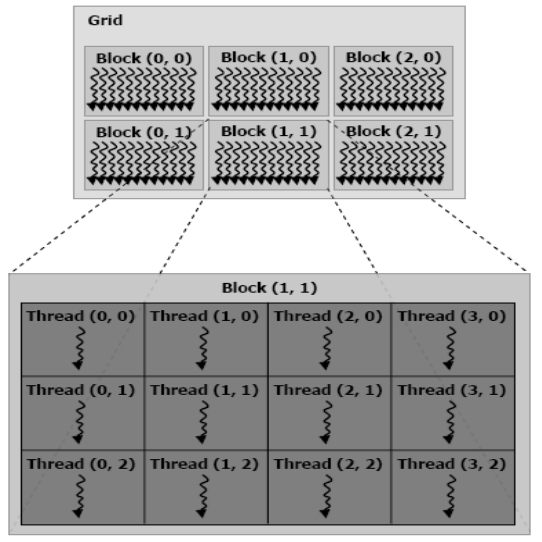
\includegraphics[width=0.45\textwidth]{figs/cap3/threads_block_grid.jpg}
	\caption{Bloques de threads organizados en una grilla de bloques \cite{rinaldi2011modelos}.}
	\label{fig:block_grid_threads}
\end{figure}

\section{Programación en CUDA C}

La programación de las GPU se lleva a cabo mediante el lenguaje \textbf{CUDA}, el cuál es una extención del lenguaje \textbf{C} debido su familiaridad y uso extendido, por lo que el lenguaje se denomina \textbf{CUDA C}. La realización de procesos en paralelos es ejecutada mediante funciones llamadas \textit{kernel} y son del tipo \textit{void}.

Existen tres tipos de funciones que se pueden llevar a cabo y son:

\begin{itemize}
	
	\item \textbf{host} función clásica de C que se ejecuta en la CPU, siendo invocable únicamente por funciones que se ejecuten en la CPU. 

	\item \textbf{global} es una función \textit{kernel} invocada desde la CPU para ejecutarse en la GPU. 
%	Debe especificar la cantidad de bloques y de \textit{threads} por bloque a lanzar la función.
	
	\item \textbf{device} es una función que se ejecuta en la GPU y únicamente puede ser llamada desde un \textit{kernel}.
	
\end{itemize}

En el presente trabajo sólo se utilizaran funciones de tipo \textbf{host} y \textbf{global}, pudiéndose realizar en un futuro el  \textit{profiling} mediante el uso de las funciones \textbf{device}.

Otra particularidad que se presenta en la programación es el manejo de la memoria; por parte del \textit{host} como del \textit{device}, siendo abordado posteriormente.
\newpage

\subsection{Programación de un \textit{kernel}}

A modo de ejemplo para poder visualizar las diferencias de programación en una función de un kernel en CUDA , con una típica función de C, se muestra la siguiente: (la cual es de la obtencion de la densidad)


{\footnotesize
	\begin{frame}{}
		\lstset{language=C,
			framesep=2mm,
			basicstyle=\ttfamily,
			keywordstyle=\color{blue}\ttfamily,
			stringstyle=\color{red}\ttfamily,
			commentstyle=\color{green}\ttfamily,
			morecomment=[l][\color{magenta}]{\#}
		}
		\begin{lstlisting}
		#include <momentoDensity.h>
		#include <stdio.h>
		
		void momentoDensity(scalar* rho, scalar* field, basicMesh* mesh) {
		
		// Suma de todas las componentes
		
		for( uint i = 0 ; i < mesh->nPoints ; i++ ) {
		
		rho[i] = 0;	    
		for( uint j = 0 ; j < mesh->Q ; j++ ) {
		rho[i] += field[ i*mesh->Q + j ];
		}		
		}
		}
		\end{lstlisting}
		
	\end{frame}
}


{\footnotesize
	\begin{frame}{}
		\lstset{language=C,
			framesep=2mm,
			basicstyle=\ttfamily,
			keywordstyle=\color{blue}\ttfamily,
			stringstyle=\color{red}\ttfamily,
			commentstyle=\color{green}\ttfamily,
			morecomment=[l][\color{magenta}]{\#}
		}
		\begin{lstlisting}
		#include <cudaMomentoDensity.h>
		#include <cuda_runtime.h>
		#include <stdio.h>
		#include <stdlib.h>
		
		extern "C" __global__ void cudaMomentoDensity(cuscalar* field,
		cuscalar* rho,
		int np,
		int Q ) {
		
		int idx = threadIdx.x + blockIdx.x*blockDim.x;	
		if( idx < np ) {	
		int j= 0;		
		cuscalar sum = 0;		
		while ( j < Q ) {		
		sum += field[ idx*Q + j ];			
		j++;			
		}				
		rho[idx] = sum;	
		}
		}
		
		\end{lstlisting}
		
	\end{frame}
}








\subsection{Utilización de la memoria de \textit{host} y \textit{device}}




La allocación de memoria en el \textit{host} es la misma que se utiliza en C: \textbf{malloc($\>$)}, mientras que en el \textit{device} se realiza mediante: \textbf{cudaMalloc($\>$)}, la cual recibe los siguientes argumentos:
{\footnotesize
\begin{frame}{}
	\lstset{language=C,
		framesep=2mm,
		basicstyle=\ttfamily,
		keywordstyle=\color{blue}\ttfamily,
		stringstyle=\color{red}\ttfamily,
		commentstyle=\color{green}\ttfamily,
		morecomment=[l][\color{magenta}]{\#}
	}
	\begin{lstlisting}
cudaMalloc(void **devPtr, size_t size);
	\end{lstlisting}

\end{frame}
}
(devPtr) puntero para allocar la memoria del \textit{device} , (size\_t) memoria en bytes a reservar. Se debe tener en cuenta que la memoria se reserva de manera lineal.

La transferencia de datos entre los dos tipos de memoria se efectua mediante la función \textbf{cudaMemcpy($\>$)}, la cual recibe los siguientes argumentos:
{\footnotesize
\begin{frame}{}
	\lstset{language=C,
		framesep=2mm,
%		baselinestretch=1.2,
		basicstyle=\ttfamily,
		keywordstyle=\color{blue}\ttfamily,
		stringstyle=\color{red}\ttfamily,
		commentstyle=\color{green}\ttfamily,
		morecomment=[l][\color{magenta}]{\#}
	}
	\begin{lstlisting}
cudaMemcpy(void *dst, void *src, size_t count, cudaMemcpyKind kind);
	\end{lstlisting}
	
\end{frame}
}
(dst) puntero con la dirección de destino de los datos, (src) puntero con la dirección de origen, (count) es la cantidad de bytes a transferir y (kind) es el tipo de transferencia a realizar\cite{zone2020cuda}. En la tabla \ref{tab:cudamemcy} se encuentran los cuatro tipos posibles de transferencia.

\begin{table}[h!]
	\centering
	\begin{tabular}{|c|c|}
		\hline
		\multicolumn{1}{|l|}{TIPO DE TRANSFEREMCIA} & \multicolumn{1}{l|}{SENTIDO DE TRANSFERENCIA} \\ \hline
		\textbf{cudaMemcpyHostToHost}               & host host                                     \\ \hline
		\textbf{cudaMemcpyHostToDevice}             & host device                                   \\ \hline
		\textbf{cudaMemcpyDeviceToHost}             & device host                                   \\ \hline
		\textbf{cudaMemcpyDeviceToDevice}           & device device                                 \\ \hline
	\end{tabular}
	\caption{Tipos de transferencias de datos en CUDA \cite{represa2016introduccion}.}
	\label{tab:cudamemcy}
\end{table}

El lanzamiento de un \textit{kernel} en varios bloques tiene una particularidad en la ejecución de los procesos, los \textit{threads} de cada bloque llevan realizan los procesos en diferentes tiempos por ser independientes. \textbf{Que quiere decir esta oracion. Parece no estarbien escrita} Para evitar problemas en las operaciones que se realizan en la memoria pasada al \textit{kernel} ( surge en parte debido a que un \textit{kernel} es una función \textbf{void} ), se utiliza la función \textbf{cudaDeviceSynchronize($\>$)}. Esta función hace que los bloques realicen su ejecución y antes de proceder a la siguiente instrucción espera a que todos los bloques de \textit{threads} hallan terminado. Para sincronizar los \textit{threads} de un mismo bloque en un función \textit{device} se utiliza \textbf{syncthreads($\>$)}.


\subsection{Ejemplo de programacion de un kernel}
















\section{Arquitectura de memoria}

\begin{figure}[h!]
	\centering
	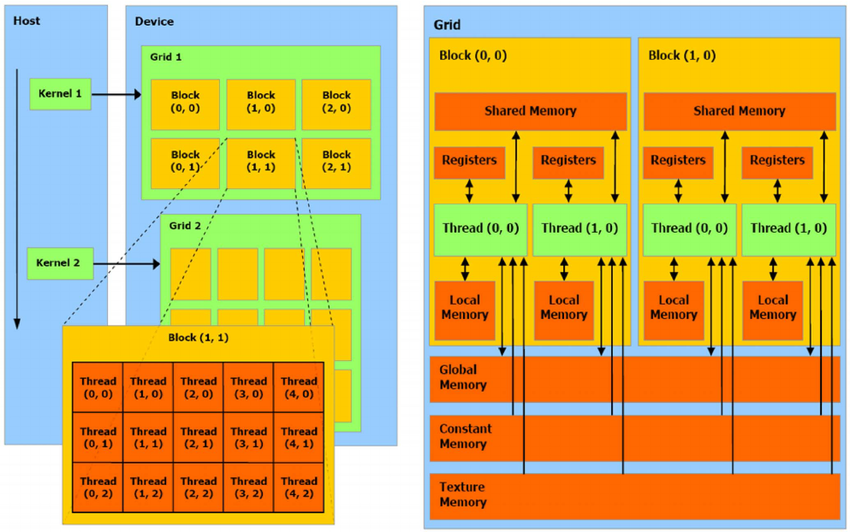
\includegraphics[width=\textwidth]{figs/cap3/Schematization-of-CUDA-architecture-Schematic-representation-of-CUDA-threads-and-memory.png}
	\caption{Esquematización de la arquitectura de CUDA. Izquierda: lanzamiento de un \textit{kernel} desde el \textit{host}. Derecha: jerarquía de memoria.  \cite{nobile2014cutauleaping}.}
	\label{fig:schedule_architecture_cuda}
\end{figure}

Según la arquitectura que posea un procesador, son su respectiva jerarquía en memoria, accesos y latencias se piensa cómo llevar a cabo la implementación de un código. Por ello es de importancia conocer éstas características. 

Se mencionó anteriormente que el \textit{host} y \textit{device} poseen su propia memoria. La transferencia de datos de una memoria a otra tiene una muy alta latencia en cualquiera de los dos sentidos. 

%Por lo que al realizar la implementación de un código hay que minimizar la transferencia para que el tiempo de ejecución de los procesos sea mínimo.

Cuando el \textit{host} efectúa su rutina de ejecución y se encuentra con un lanzamiento de \textit{kernel}, éste será llevado a cabo en múltiples \textit{threads} del \textit{device}. Una representación de ello se muestra en la figura \ref{fig:schedule_architecture_cuda}. 

Los procesos en el \textit{device} tienen almacenados los datos según una jerarquía de memoria, con su respectiva limitación de acceso que se observa en la figura \ref{fig:schedule_architecture_cuda}. Los \textit{threads} pueden acceder a datos de muchas memorias diferentes en distintos procesos, dichas memorias son las siguientes:

\begin{itemize}
	\item  \textit{register memory} es visible para un único \textit{thread}
	\item \textit{local memory} tiene las mismas caracteísticas que \textit{register memory} pero con una performance menor.
	\item \textit{shared memory} es visible por todos los \textit{threads} de un mismo bloque, posee una baja latencia en su acceso.
	\item \textit{global memory} es visible por todos los \textit{threads} de la grilla y también por el \textit{host}, posee una alta latencia de acceso.
	
	Las siguientes memorias poseen una alta latencia de acceso son asignadas y son aignadas para usos específicos y generalmente se almacenan en \textit{caché}:
	
	\item \textit{constant memory} es visible por todos los \textit{threads} de la grilla siendo únicamente de lectura. El uso de ésta memoria puede reducir el ancho de banda de memoria requerido en comparación con la {global memory}
	\item \textit{texture memory} es otra memoria en la que sólo se puede leer y tienen acceso todos los \textit{threads} de la grilla. Al realizar lecturas de \textit{threads} ó \textit{threadblocks} adyacentes su performance en comparación con \textit{global memory} es mayor. 
	
\end{itemize}




\textbf{yo agregaria aca que este codigo compilado puede usarse en Python, y decir algo general de como hay que compilarso e importarlo con PyCUDA}

%%% Local Variables: 
%%% mode: latex
%%% TeX-master: "template"
%%% End: 
